% Chapter 6

\chapter{Rechargeable aluminium-ion batteries using oxides and other materials as cathodes} % Main chapter title
In this chapter, we discuss performance of AIBs using other materials, which have been previously used in other battery technologies, and make an attempt to establish their mechanism in a new system.
\label{chap6} % For referencing the chapter elsewhere, use \ref{Chapter1} 

%----------------------------------------------------------------------------------------

% Define some commands to keep the formatting separated from the content 
\newcommand{\keyword}[1]{\textbf{#1}}
\newcommand{\tabhead}[1]{\textbf{#1}}
\newcommand{\code}[1]{\texttt{#1}}
\newcommand{\file}[1]{\texttt{\bfseries#1}}
\newcommand{\option}[1]{\texttt{\itshape#1}}

%----------------------------------------------------------------------------------------
\section{Theory and background}
\subsection*{\ce{MoS2} nanoflowers}
\subsection*{\ce{MoSe2} nanoflowers}
 \begin{figure}[tbh!]
  \centering
  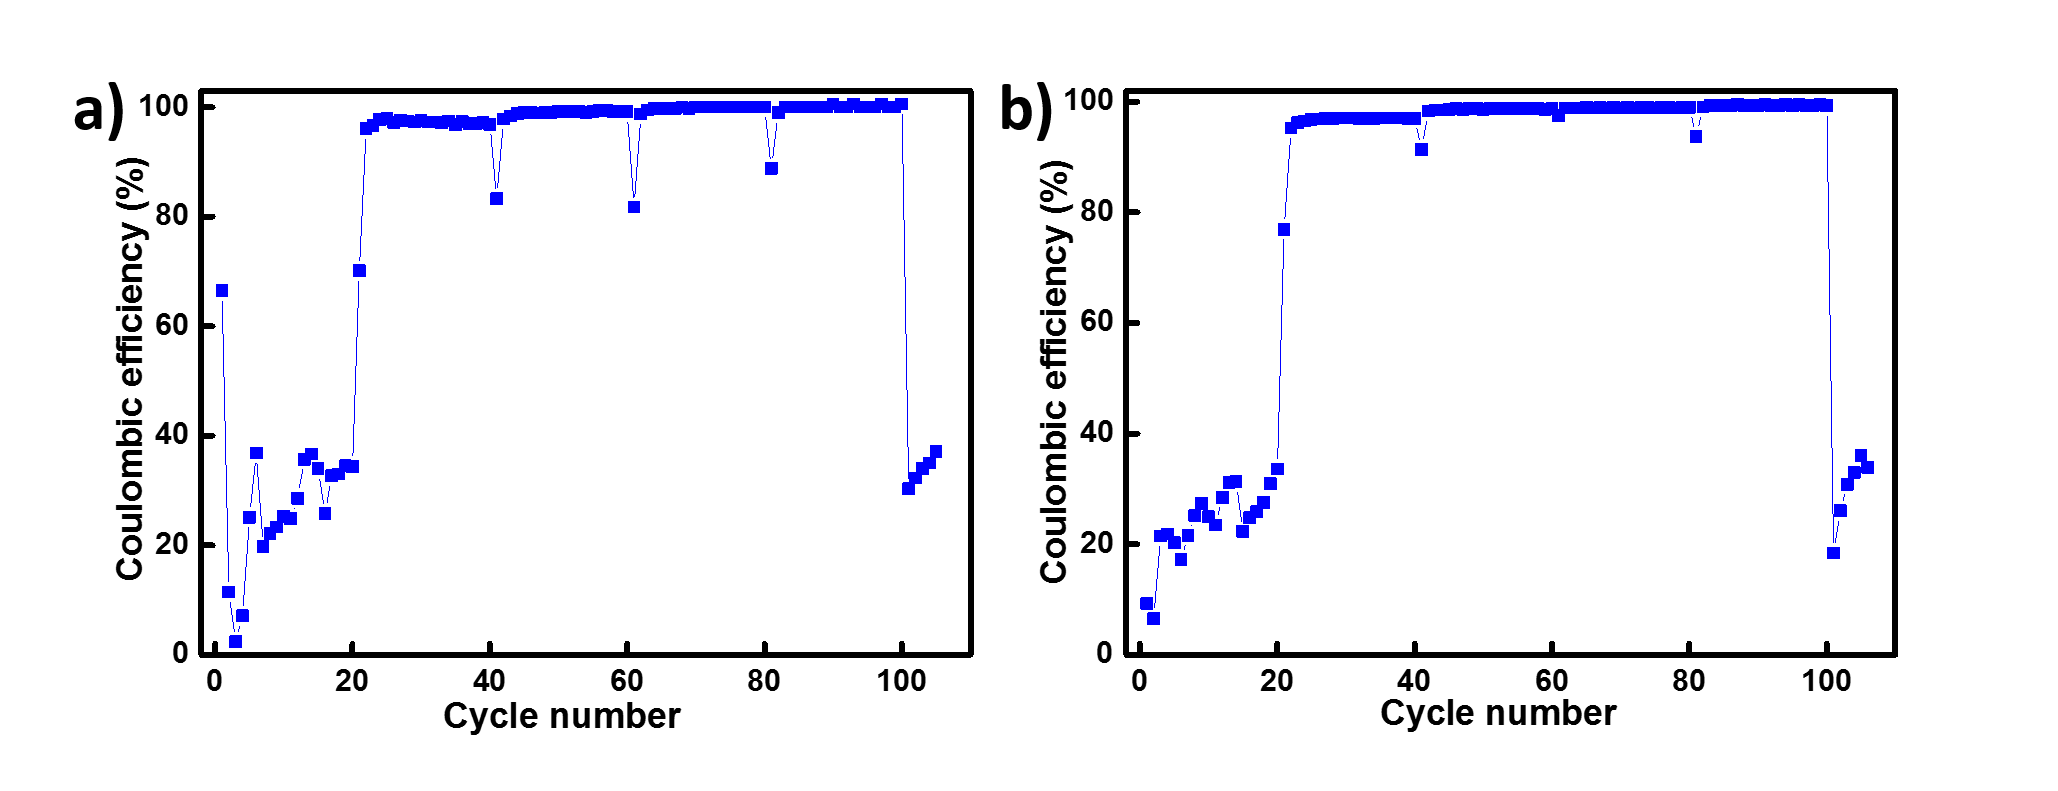
\includegraphics[width=\textwidth]{Figures/chap6fig/MoX2YNCEs}
    \caption{Crystal structure of \ce{SnO2}. a) Tetragonal unit cell with space group P4/nmm and space group number 129. b) Top view of the crystal lattice.}
  \label{Figures/chap6fig:MoX2YNCEs}
\end{figure}
 \begin{figure}[tbh!]
  \centering
  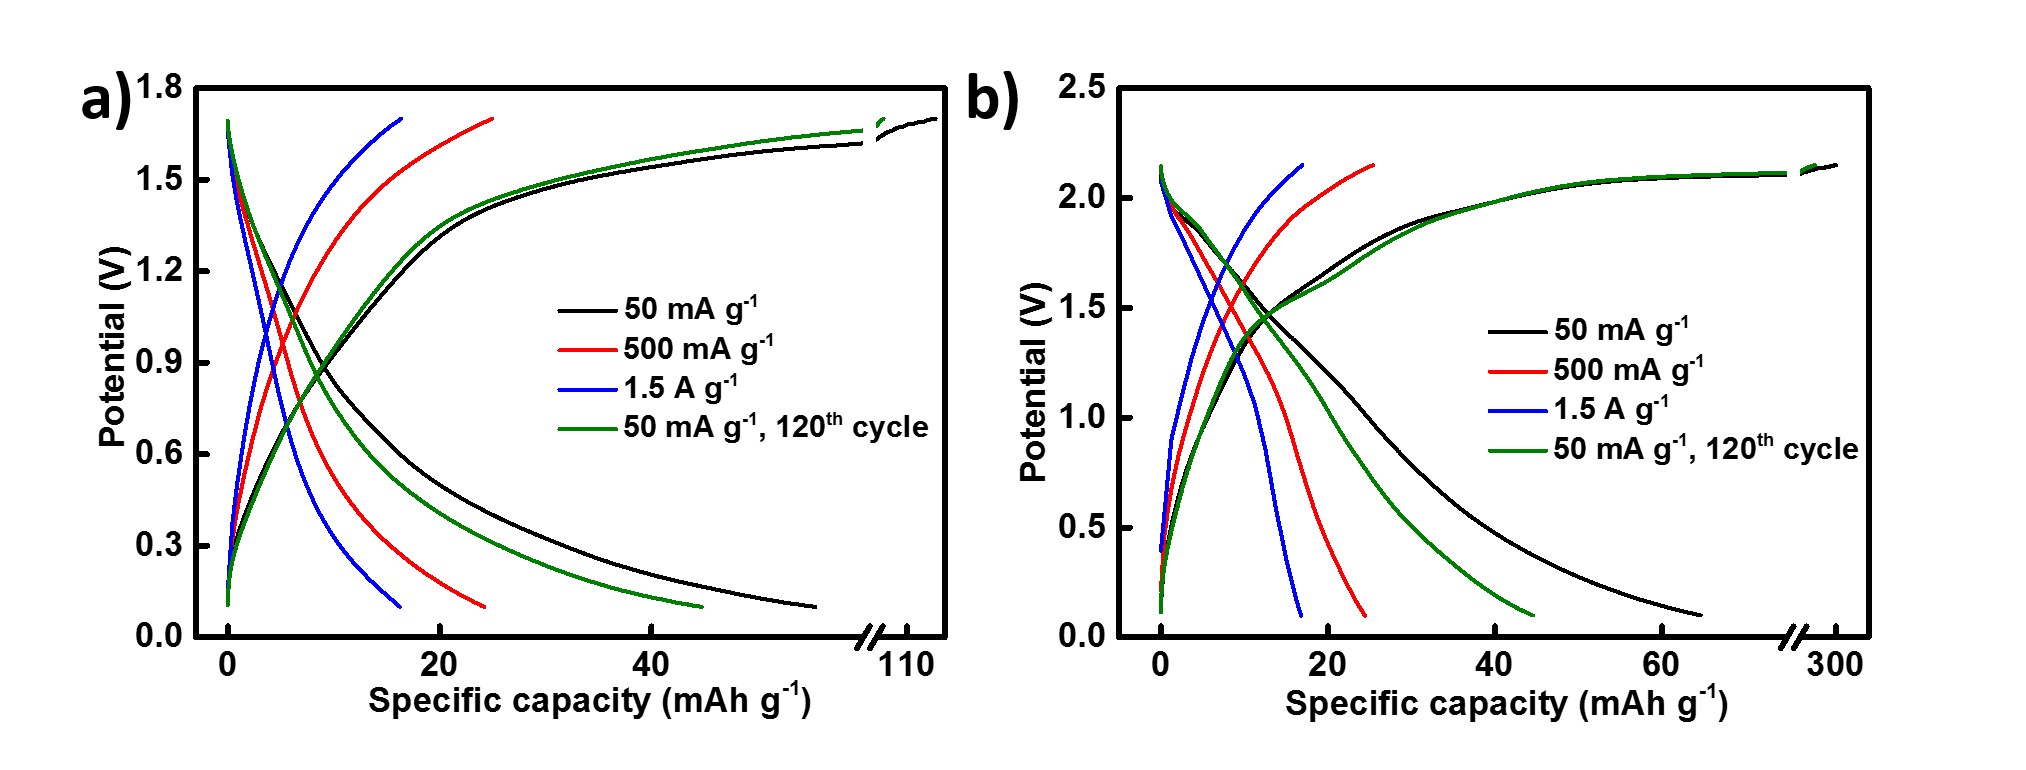
\includegraphics[width=\textwidth]{Figures/chap6fig/MoX2YNCDCs}
    \caption{Crystal structure of \ce{SnO2}. a) Tetragonal unit cell with space group P4/nmm and space group number 129. b) Top view of the crystal lattice.}
  \label{Figures/chap6fig:MoX2YNCDCs}
\end{figure}
\subsection*{Tin oxide, \ce{SnO2}}
Tin, (Sn). has been a popular choice in energy storage devices due to its unique physical and chemical properties. Sn has high conductivity and a good thermal and mechanical stability. It is inexpensive and non-toxic. With a high theoretical capacity of 992 mAh g$^{-1}$, it can prove to be a very good battery electrode material. In lithium-ion batteries, it forms \ce{Li4.4Sn} stoichiometry in a fully lithiated state. The reversible reaction that takes place is as follows:
\begin{center}
    xLi + x\ce{e-} + ySn $\longleftrightarrow$ Li$_X$Sn  
\end{center}
Yet, the performance deteriorates when it is used as an active battery material. The electrical conductivity and electrochemical stability decreases. It undergoes high volumetric expansion during the lithiation process with a volume change of 200\%. Sn starts to aggregate leading to cathode pulverisation and capacity fading \cite{park_effect_2008, zhao_tin-based_2016}.  
Tin (+IV) oxide is an inorganic compound with the formula \ce{SnO2}. It finds abundant use as a colorant, polishing powder, for glass coatings and as a sensor for combustible gases. Due to its high theoretical capacity ($\approx$ 782mAh g$^{-1}$), safe handling and environmental-friendliness, \ce{SnO2} is a good battery material. Miyasak \textit{et al.} used tin-based amorphous composite oxide (TCO) containing Sn(II)-O as the active center for lithium-insertion, which made an oxide network \cite{idota_tin-based_1997}. However, \ce{SnO2} also underwent large volumetric changes $\approx$ 300{\%}, which caused slow diffusion kinetics. After continuous charge-discharge cycles, cathodes experienced similar degradation and capacity reduction. To improve the battery performance, carbonaceous materials were added to \ce{SnO2}; carbon does not form tin carbide. It not only increased the surface area, which allows more lithiation to take place but also controlled the volume expansion/shrinkage. Additionally, it improved the conductivity of the material \cite{nowak_composites_2018}. Lee \textit{et al.} obtained synthetic graphite modified by a highly dispersed tin oxide which improved the cell's performance \cite{navarro-suarez_2d_nodate}. 
It was observed that carbon coating on \ce{SnO2} surface prevents their agglomeration and volume expansion. A smaller particle size (like nanorods\cite{liu_direct_2009}, nanobelts\cite{duan_single_2005}, , nanowires\cite{huang_situ_2010}, nanotubes\cite{wang_large-scale_2011}, or/and a porous structure of the active material would further increase the contact area between the electrode and the electrolyte, accelerating the transport of ions and improve its capacity. 
However, it was important to find out if \ce{SnO2} worked in an aluminium-ion cell. SO, we tested \ce{SnO2} as a cathode for AIBs. The graph obtained was similar with Li/\ce{SnO2} cells.  
 \begin{figure}[tbh!]
  \centering
  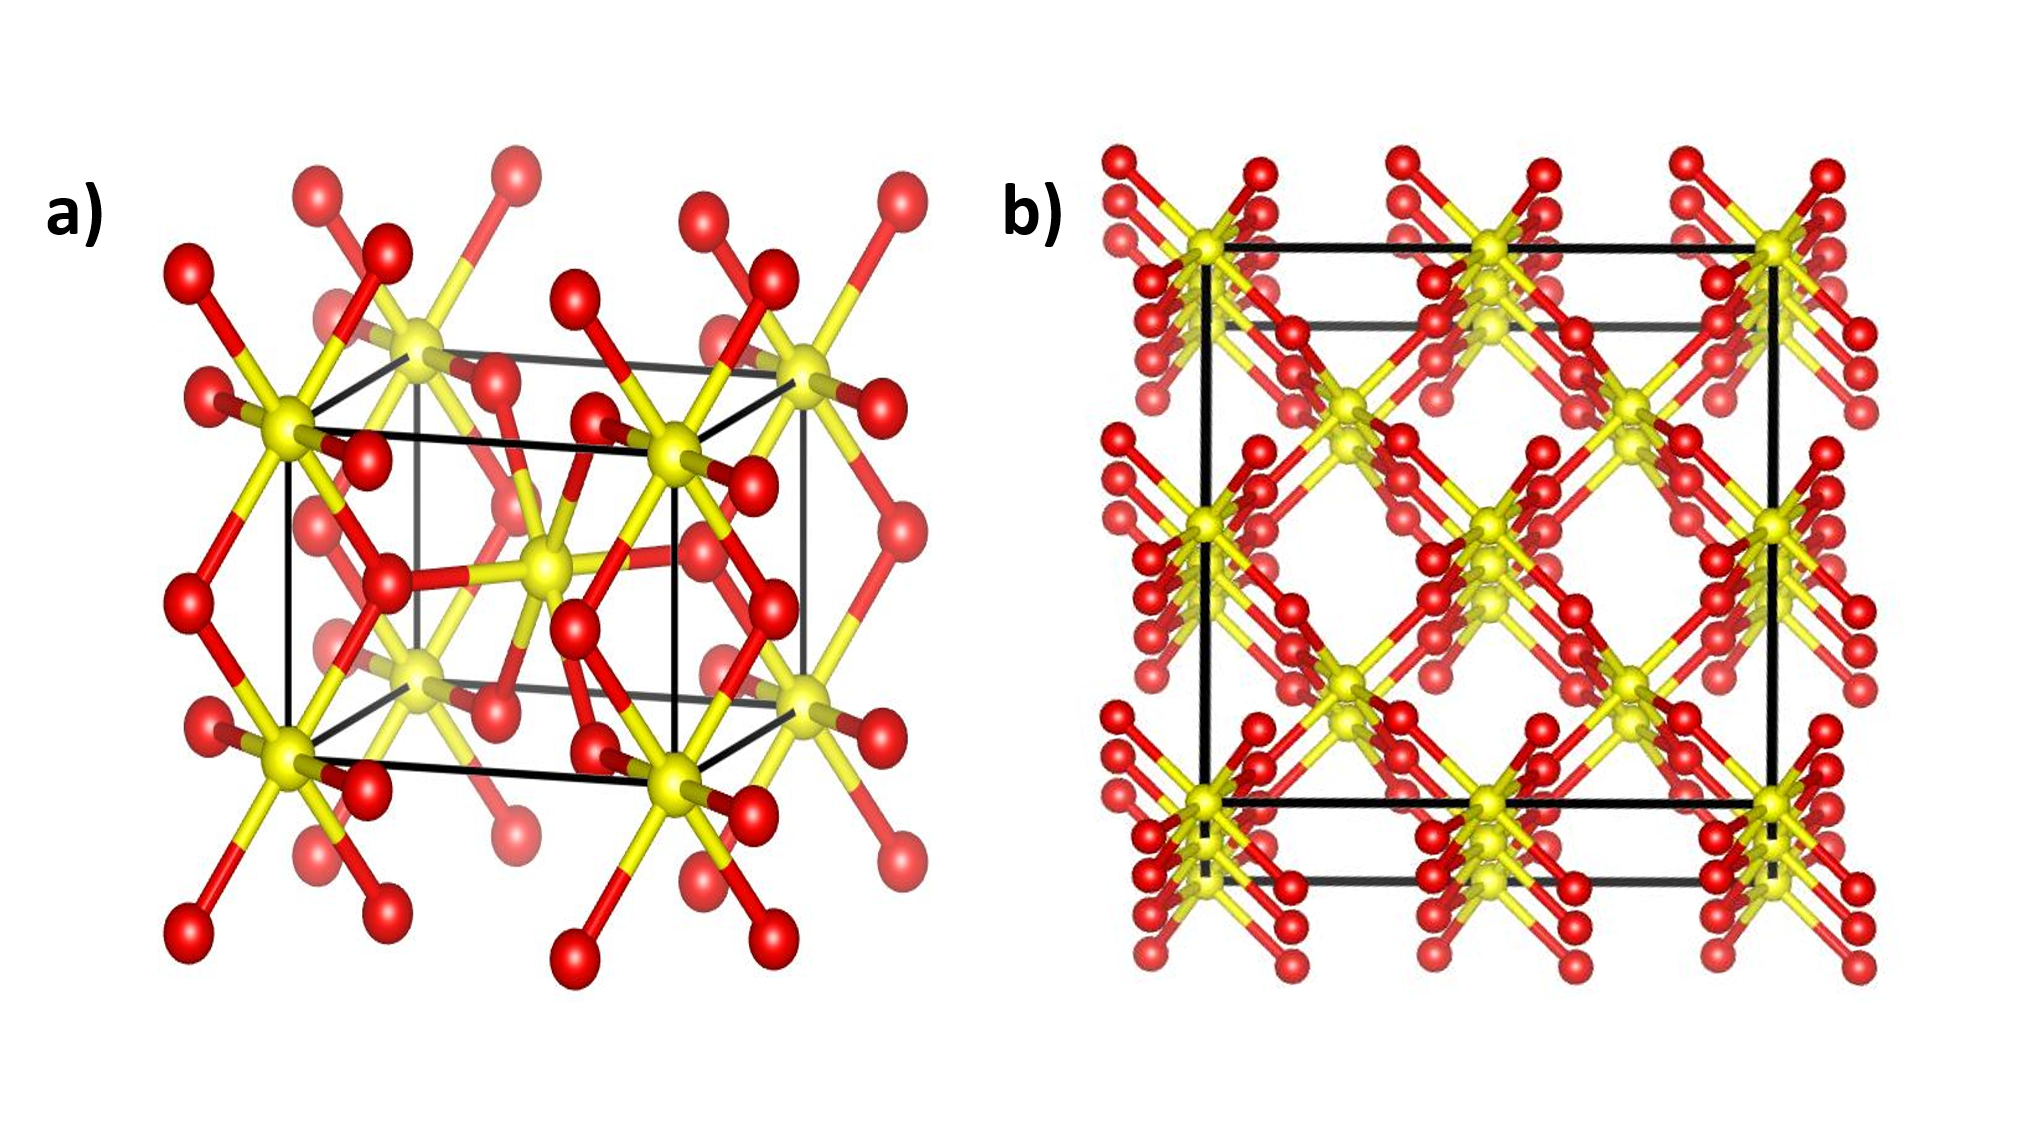
\includegraphics[width=\textwidth]{Figures/chap6fig/SnO2crys}
    \caption{Crystal structure of \ce{SnO2}. a) Tetragonal unit cell with space group P4/nmm and space group number 129. b) Top view of the crystal lattice.}
  \label{Figures/chap6fig:SnO2crys}
\end{figure}
 \begin{figure}[tbh!]
  \centering
  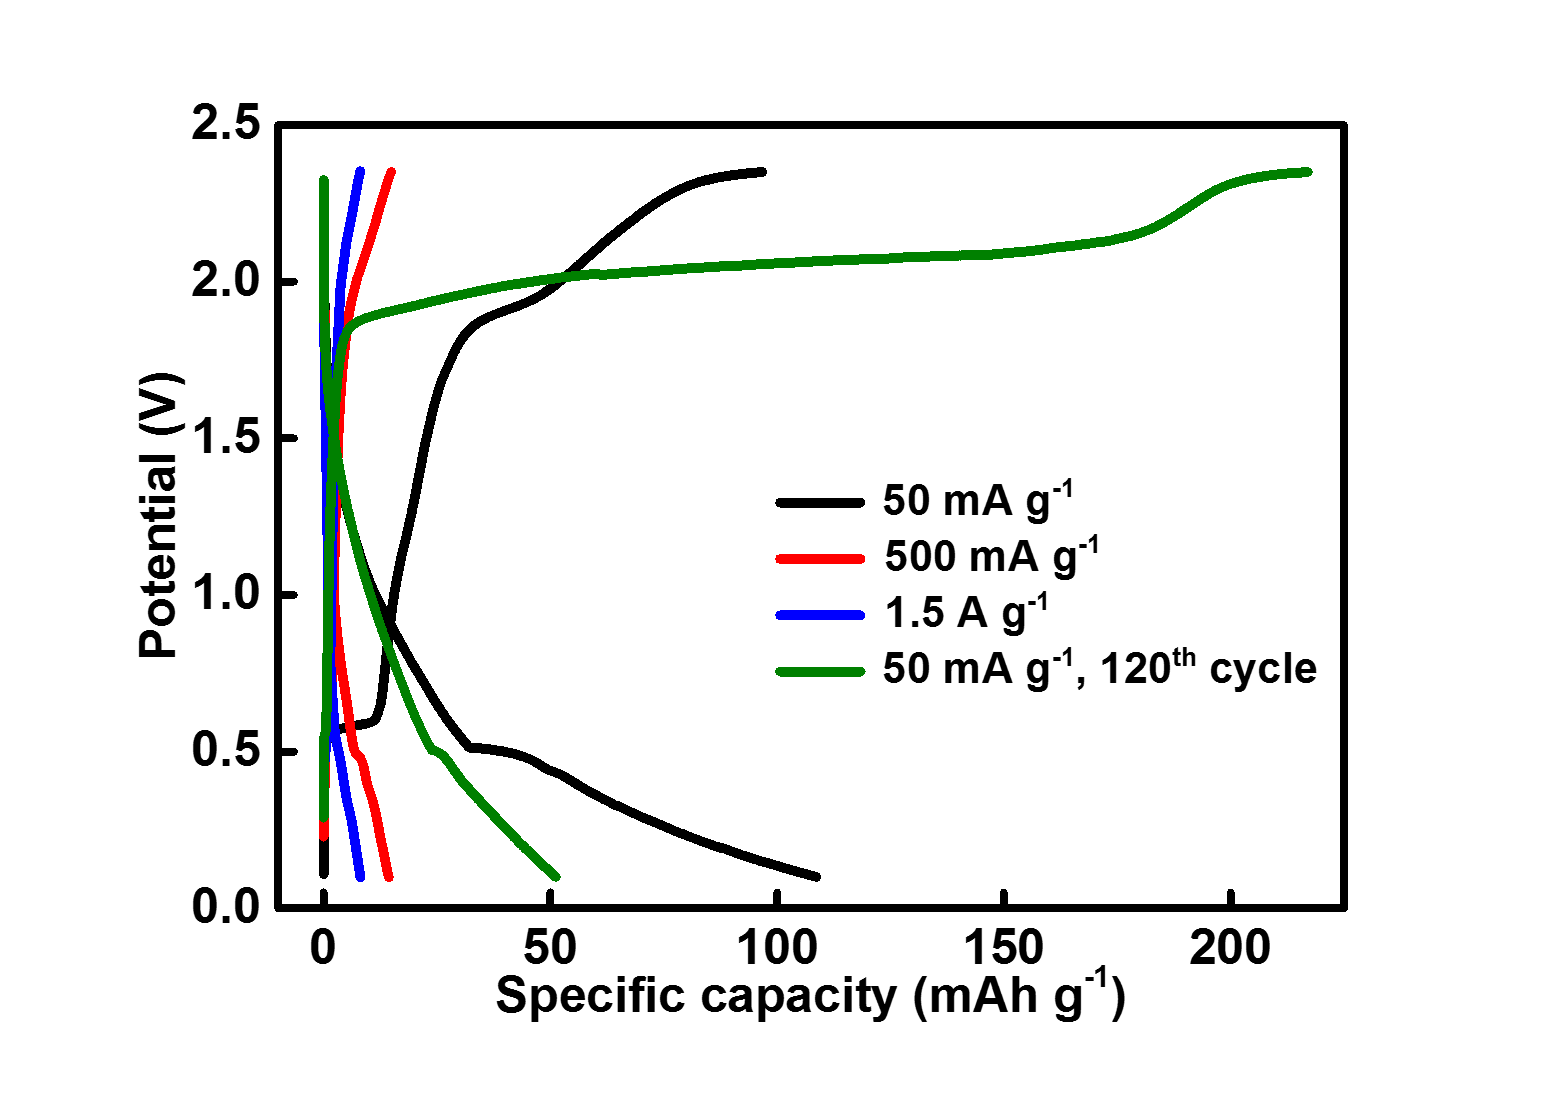
\includegraphics[width=\textwidth]{Figures/chap6fig/SnO2CDC}
    \caption{Galvanostatic cycle test of an Al/\ce{SnO2} cell in a two-electrode setup at various current rates..}
  \label{Figures/chap6fig:SnO2CDC}
\end{figure}

\subsection*{Molybdenum trioxide, \ce{MoO3}}
Molybdenum trioxide, \ce{MoO3} is an intermediate formed during production of Mo metal. It is an industrial catalyst for acrylonitrile via oxidation of propene and ammonia. It consists of layers of \ce{MoO6} octahedra held together by covalent forces in the (100) and (001) directions and by Van der Waals forces in the (010) direction, Figure \ref{Figures/chap6fig:MoO3crys}a and b. Its layered structure makes it a very good battery material (an easier intercalation/ deintercalation) and a straightforward \ce{Mo^{4+}}/\ce{Mo^{5+}} coupling. When used in LIBs, it might undergo an insertion/ extraction process or a conversion reaction for lithium storage. It has been seen that high concentrations of unsolvated \ce{Li+} in the oxide host lattice causing significant irreversible structural and morphological changes resulting in capacity fading. 
 \begin{figure}[tbh!]
  \centering
  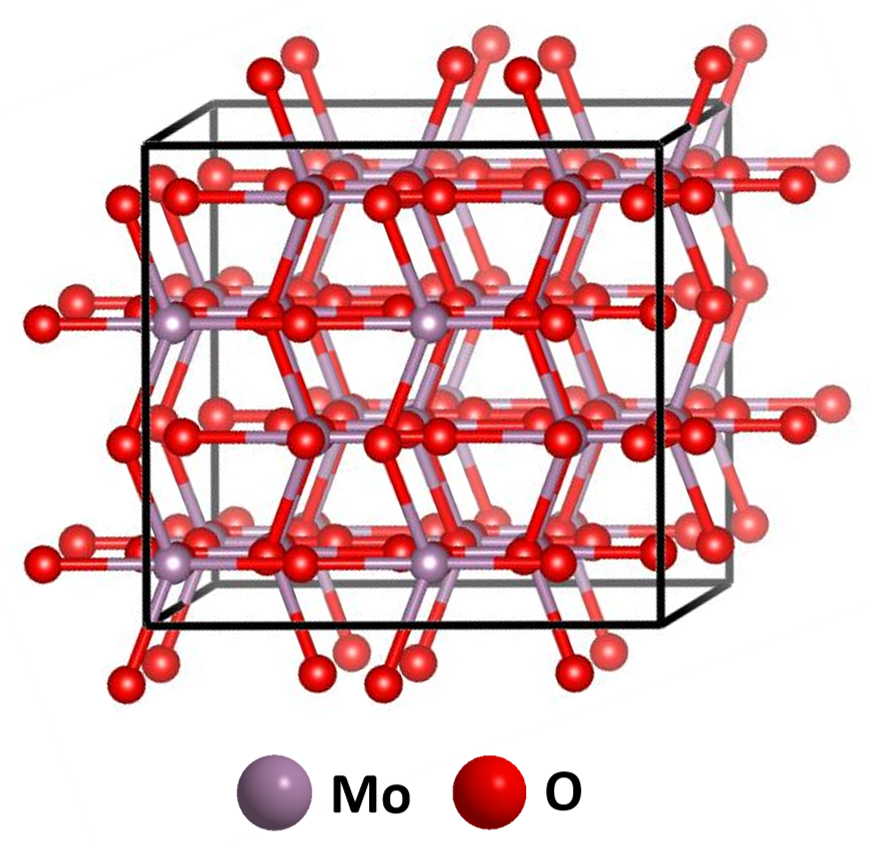
\includegraphics[width=\textwidth]{Figures/chap6fig/MoO3crys}
    \caption{Crystal structure of \ce{MoO3}. a) Tetragonal unit cell with space group P4/nmm and space group number 129. b) Top view of the crystal lattice.}
  \label{Figures/chap6fig:MoO3crys}
\end{figure}
 \begin{figure}[tbh!]
  \centering
  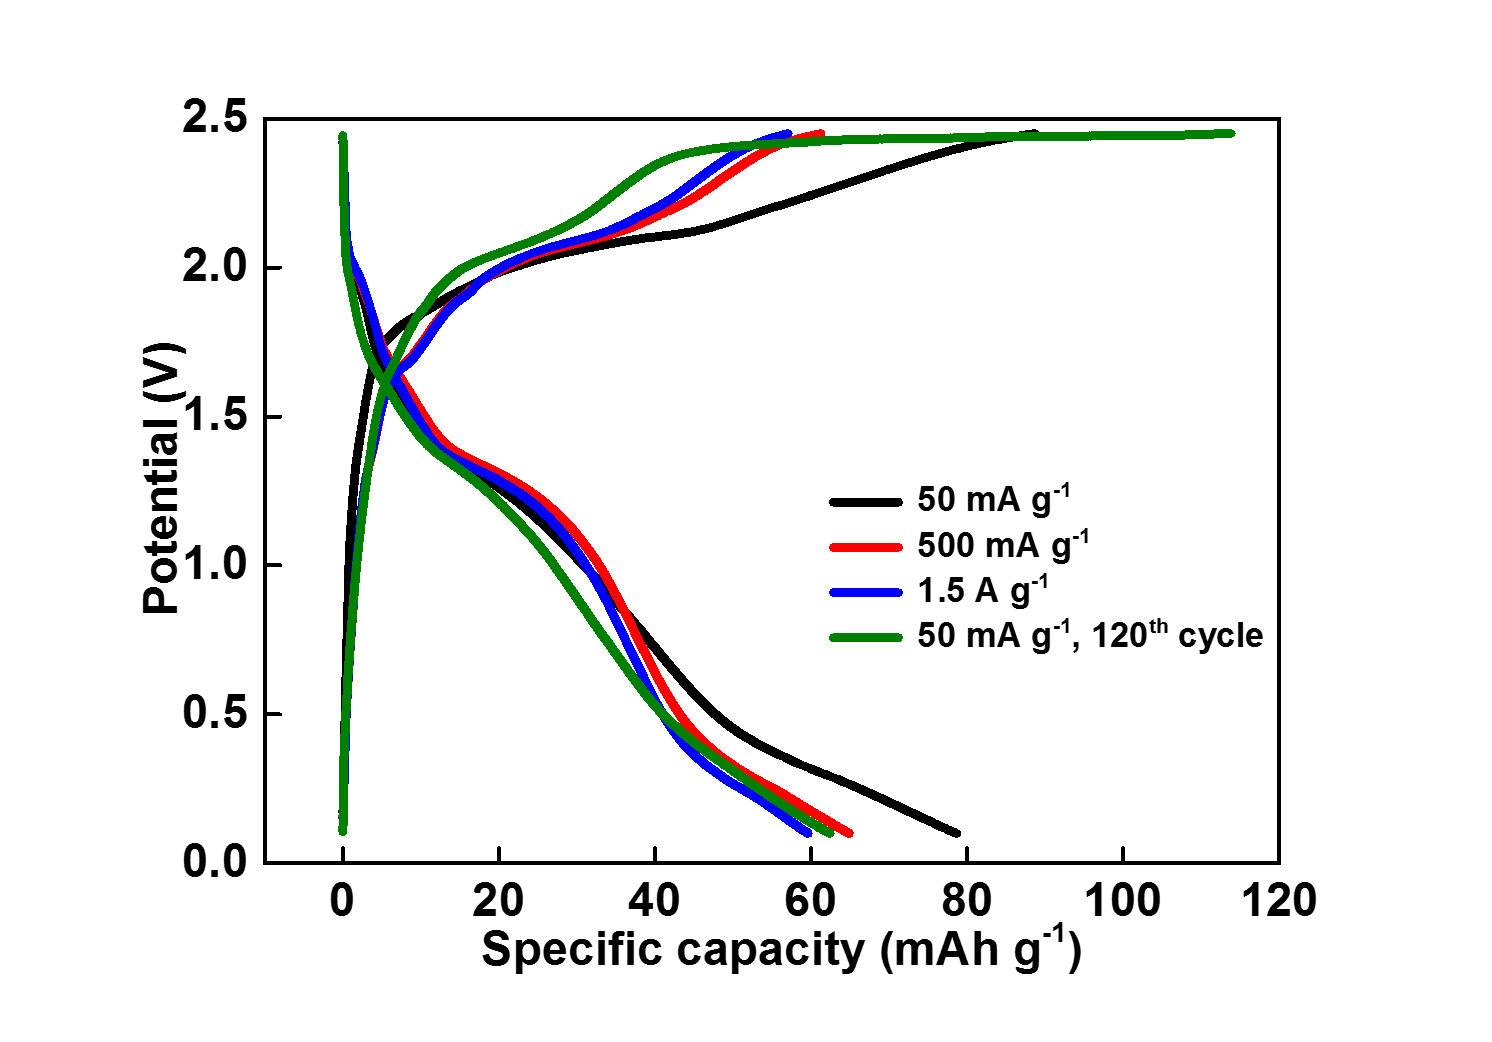
\includegraphics[width=\textwidth]{Figures/chap6fig/MoO3CDCredo}
    \caption{Galvanostatic cycle test of an Al/\ce{MoO3} cell in a two-electrode setup at various current rates.}
  \label{Figures/chap6fig:MoO3CDCredo}
\end{figure}

\subsection*{Graphitic Carbon Nitride, g-\ce{C3N4}}
high intrinsic photoabsorption and photo-responsiveness, semi-conductive properties, high stability under physiological conditions, and good bio-compatibility







\subsection*{Prussian blue, \ce{C19Fe7N18}}
Prussian blue was originally commercialised in the dye industry. Since, it has been used for electrolysis, thermal power generation and energy storage. It has a face-centred cubic lattice with an open framework as shown in Figure \ref{Figures/chap6fig:pbcrys}, which helps in insertion of ions in the sub-cages. Its structure is very stable and has a number of redox sites present. Each molecular formula contains two redox centres \ce{M+2}/\ce{M3+}, where M is any transition metal (Fe, Co, Ni, Mn, Cu, Zn). It reaches 2\ce{e-} redox capacity after reversibly intercalating 2 monovalent alkali ions per molecular unit. Presence of large lattice interstices and ionic channels renders a high specific capacity. 







 \begin{figure}[tbh!]
  \centering
  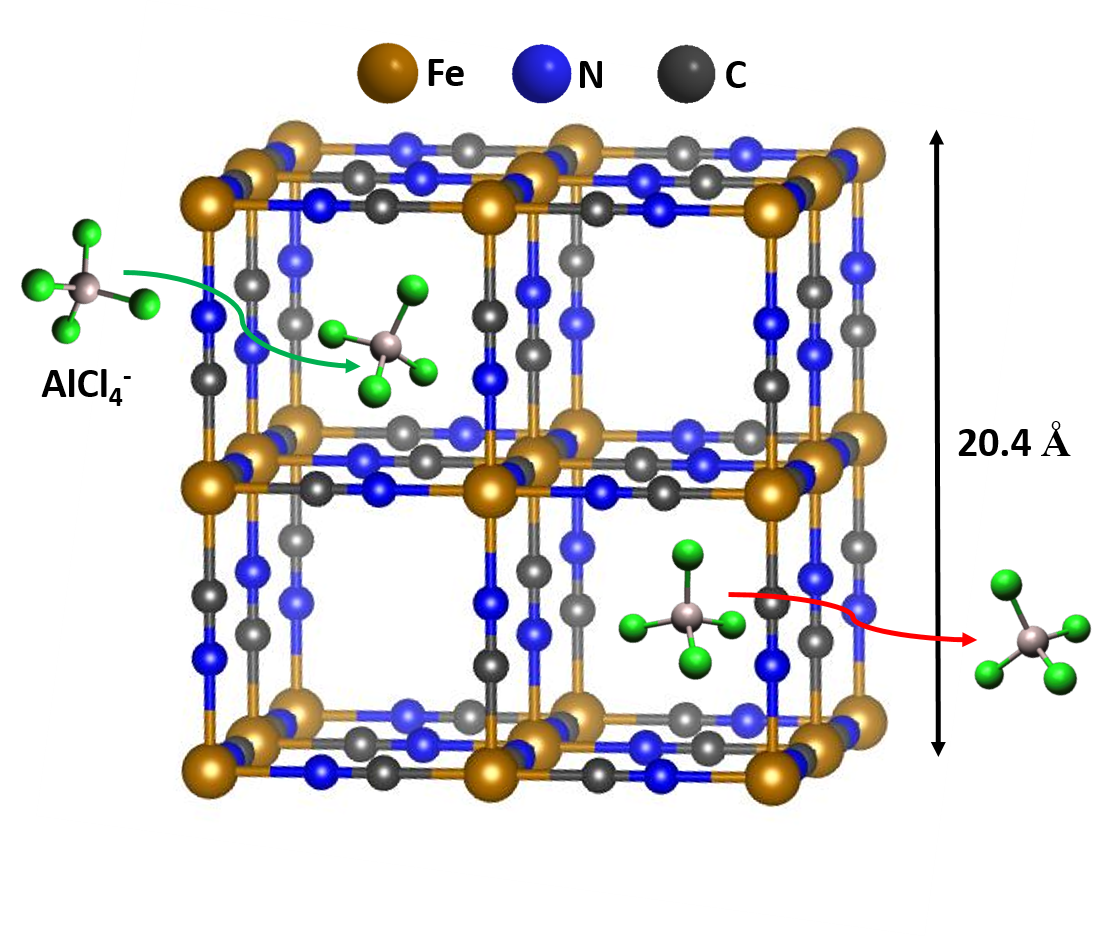
\includegraphics[width=\textwidth]{Figures/chap6fig/pbcrys}
    \caption{Crystal structure of prussian blue a) Tetragonal unit cell with space group P4/nmm and space group number 129. b) Top view of the crystal lattice.}
  \label{Figures/chap6fig:pbcrys}
\end{figure}
 \begin{figure}[tbh!]
  \centering
  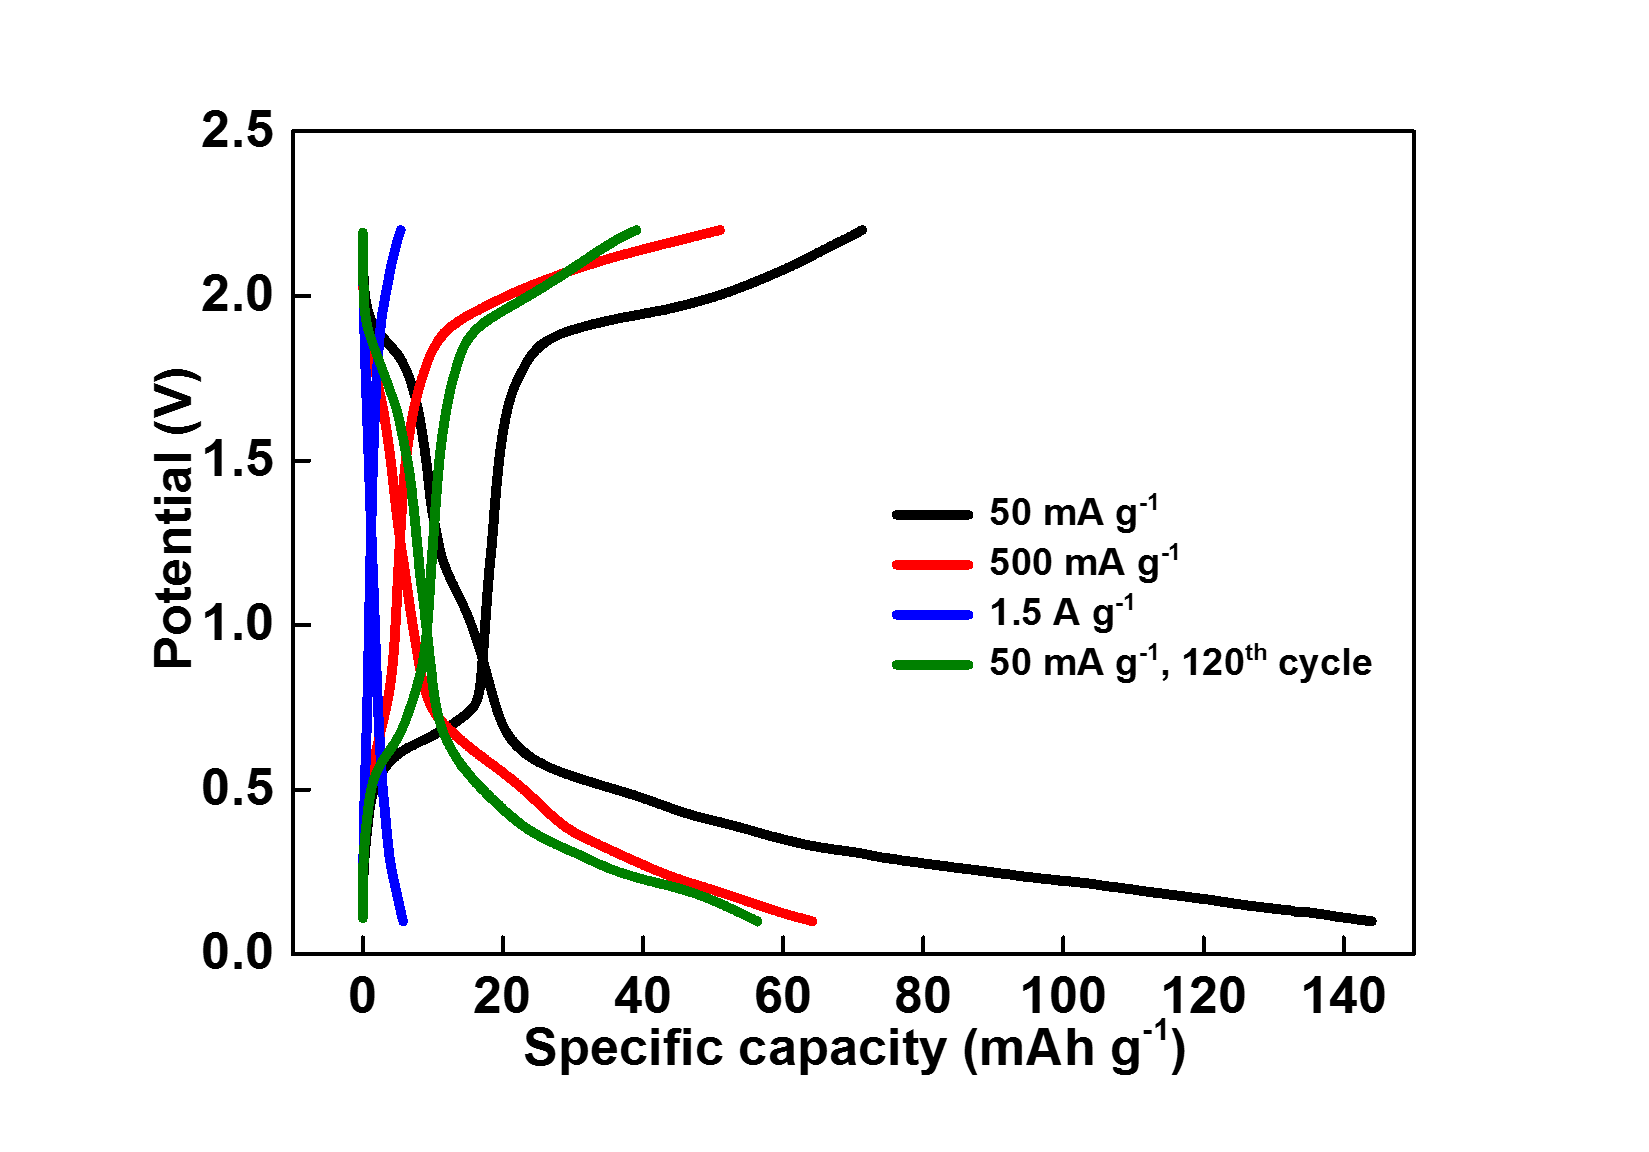
\includegraphics[width=\textwidth]{Figures/chap6fig/pbCDC}
    \caption{Galvanostatic cycle test of an Al/\ce{C19Fe7N18} cell in a two-electrode setup at various current rates.}
  \label{Figures/chap6fig:pbCDC}
\end{figure}





\section{Experimental methods}
Same as discussed in Chapter\ref{chap3}.
\section{Results and discussions}
\subsection*{}






\section{Conclusion and future outlook}